%
% teil3.tex -- Beispiel-File für Teil 3
%
% (c) 2020 Prof Dr Andreas Müller, Hochschule Rapperswil
%
% !TEX root = ../../buch.tex
% !TEX encoding = UTF-8
%
\subsection{Evaluation
\label{buch:paper:varalg:subsection:evaluation}}
\index{Evaluation}%
Dieser Schritt befasst sich mit der Auswertung der einzelnen 
Permutationen. Die Berechnung wird unter anderem auch als Fitnessfunktion benannt.
Was die Fitnessfunktion zurückgibt, ist abhängig vom Ziel der Lösung.

\subsubsection{Evaluation auf das TSP angepasst
\label{buch:paper:varalg:subsection:evaluation_tsp}}
Beim Travelling-Salesman-Problem kommt es auf die Streckenlänge an, 
daher wird zur Streckenberechnung die gleiche Formel \eqref{eq:bruteforce_min_formula},
wie in der Bruteforce-Methode, angewendet.
\begin{figure}
	\centering
	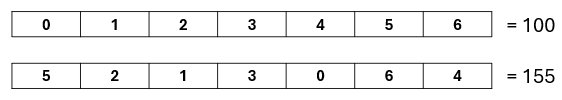
\includegraphics[width=0.8\textwidth]{
        papers/varalg/images/teil3/03GeneticStringCitiesResults.png
        }
	\caption{Beispiel eines genetischen Strings mit Ergebnissen}
	\label{fig:cities_genetic_string_results}
\end{figure}
